\PassOptionsToPackage{dvipsnames}{xcolor}
\documentclass[border=0mm]{standalone}
\usepackage[dvipsnames]{xcolor}
\usepackage{amsmath}
\usepackage{amssymb}
\usepackage{dsfont}
\usepackage{bm}
\usepackage{tikz}
\usetikzlibrary{arrows}
\usetikzlibrary{calc}
\usetikzlibrary{shapes}
\usepackage{upgreek}

\usepackage{esvect}
\newcommand{\cev}[1]{\reflectbox{\ensuremath{\vv{\reflectbox{\ensuremath{#1}}}}}}


\definecolor{color1}{rgb}{0,0.4470,0.7410}
\definecolor{color2}{rgb}{0.8500,0.3250,0.0980}
\definecolor{color3}{rgb}{0.9290,0.6940,0.1250}
\definecolor{color4}{rgb}{0.4940,0.1840,0.5560}
\definecolor{color5}{rgb}{0.4660,0.6740,0.1880}
\definecolor{lightblue}{RGB}{86,192,150}

\pgfdeclarelayer{background layer}
\pgfdeclarelayer{foreground layer}
\pgfsetlayers{background layer,main,foreground layer}


\begin{document}



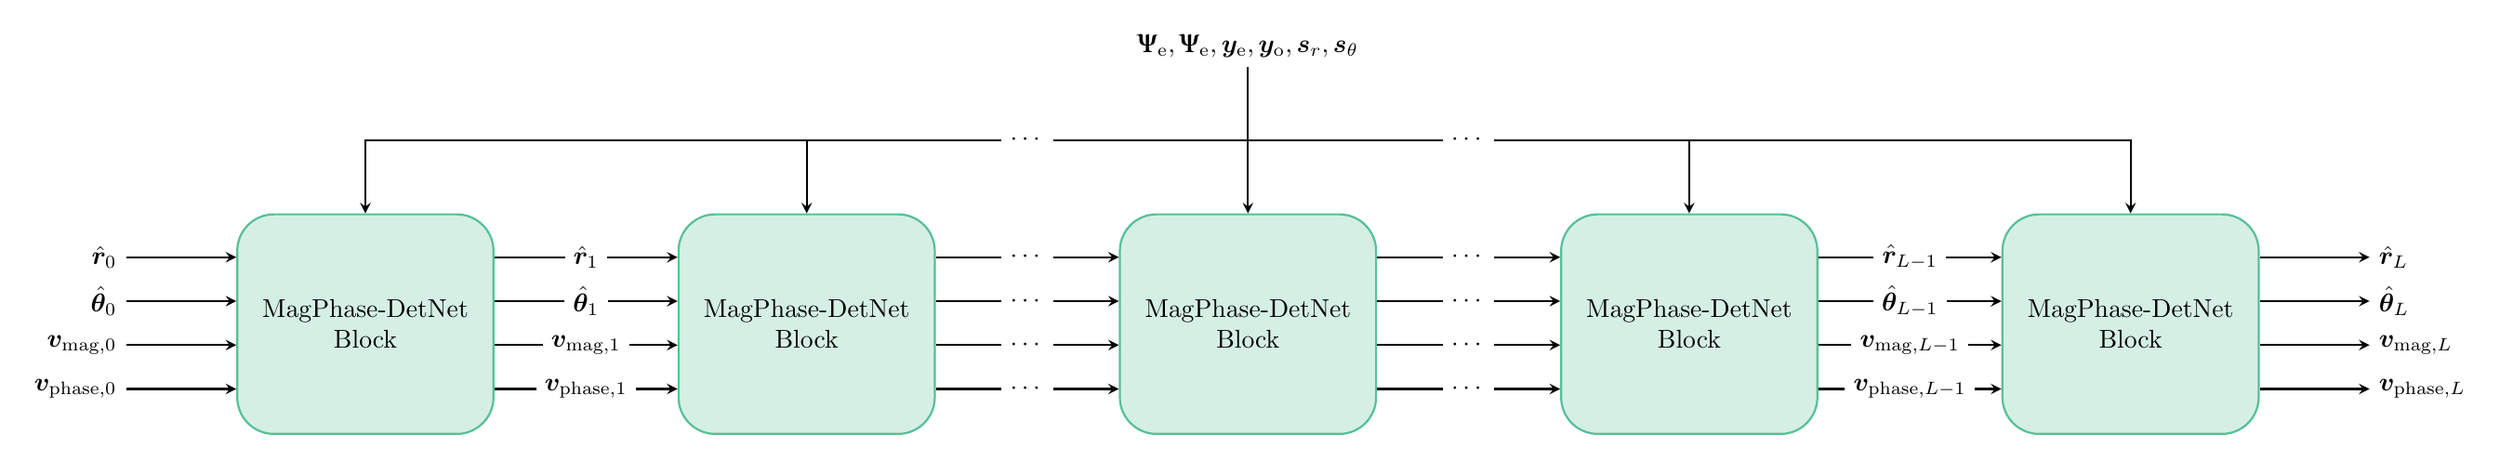
\begin{tikzpicture}[>=stealth,thick]

\node [fill=lightblue!25,rectangle, draw=lightblue, text width = 3cm, align=center, minimum width = 3.5cm, minimum height = 3cm, anchor=west,rounded corners=0.5cm] (b1) at (0,0) {MagPhase-DetNet\\ Block};

\node [fill=lightblue!25,rectangle, draw=lightblue, text width = 3cm, align=center, minimum width = 3.5cm, minimum height = 3cm, anchor=west,rounded corners=0.5cm] (b2) at ($(b1.east)+(2.5,0)$) {MagPhase-DetNet\\ Block};

\node [fill=lightblue!25,rectangle, draw=lightblue, text width = 3cm, align=center, minimum width = 3.5cm, minimum height = 3cm, anchor=west,rounded corners=0.5cm] (b3) at ($(b2.east)+(2.5,0)$) {MagPhase-DetNet\\ Block};

\node [fill=lightblue!25,rectangle, draw=lightblue, text width = 3cm, align=center, minimum width = 3.5cm, minimum height = 3cm, anchor=west,rounded corners=0.5cm] (b4) at ($(b3.east)+(2.5,0)$) {MagPhase-DetNet\\ Block};

\node [fill=lightblue!25,rectangle, draw=lightblue, text width = 3cm, align=center, minimum width = 3.5cm, minimum height = 3cm, anchor=west,rounded corners=0.5cm] (b5) at ($(b4.east)+(2.5,0)$) {MagPhase-DetNet\\ Block};



\node [anchor=east] (r1) at ($(b1.north west)+(-1.5,-0.6)$) {$\hat{\bm r}_0$};
\node [anchor=east] (theta1) at ($(b1.north west)+(-1.5,-1.2)$) {$\hat{\bm\theta}_0$};
\node [anchor=east] (vmag1) at ($(b1.north west)+(-1.5,-1.8)$) {$\bm v_{\text{mag},0}$};
\node [anchor=east] (vphase1) at ($(b1.north west)+(-1.5,-2.4)$) {$\bm v_{\text{phase},0}$};


\draw [->] (r1) -- (r1-| b1.west);
\draw [->] (theta1) -- (theta1-| b1.west);
\draw [->] (vmag1) -- (vmag1-| b1.west);
\draw [->] (vphase1) -- (vphase1-| b1.west);


\draw[->] (r1-| b1.east) -- node [midway,fill=white] {$\hat{\bm r}_{1}$} (r1-| b2.west);
\draw[->] (theta1-| b1.east) -- node [midway,fill=white] {$\hat{\bm \theta}_{1}$} (theta1-| b2.west);
\draw[->] (vmag1-| b1.east) -- node [midway,fill=white] {$\bm v_{\text{mag},1}$} (vmag1-| b2.west);
\draw[->] (vphase1-| b1.east) -- node [midway,fill=white] {$\bm v_{\text{phase},1}$} (vphase1-| b2.west);

\draw[->] (r1-| b2.east) -- node [midway,fill=white] (d1) {$\dotsb$} (r1-| b3.west);
\draw[->] (theta1-| b2.east) -- node [midway,fill=white] {$\dotsb$} (theta1-| b3.west);
\draw[->] (vmag1-| b2.east) -- node [midway,fill=white] {$\dotsb$} (vmag1-| b3.west);
\draw[->] (vphase1-| b2.east) -- node [midway,fill=white] {$\dotsb$} (vphase1-| b3.west);

\draw[->] (r1-| b3.east) -- node [midway,fill=white] (d2) {$\dotsb$} (r1-| b4.west);
\draw[->] (theta1-| b3.east) -- node [midway,fill=white] {$\dotsb$} (theta1-| b4.west);
\draw[->] (vmag1-| b3.east) -- node [midway,fill=white] {$\dotsb$} (vmag1-| b4.west);
\draw[->] (vphase1-| b3.east) -- node [midway,fill=white] {$\dotsb$} (vphase1-| b4.west);

\draw[->] (r1-| b4.east) -- node [midway,fill=white] {$\hat{\bm r}_{L-1}$} (r1-| b5.west);
\draw[->] (theta1-| b4.east) -- node [midway,fill=white] {$\hat{\bm \theta}_{L-1}$} (theta1-| b5.west);
\draw[->] (vmag1-| b4.east) -- node [midway,fill=white] {$\bm v_{\text{mag},L-1}$} (vmag1-| b5.west);
\draw[->] (vphase1-| b4.east) -- node [midway,fill=white] {$\bm v_{\text{phase},L-1}$} (vphase1-| b5.west);


\node [anchor=west] (r5) at ($(b5.north east)+(1.5,-0.6)$) {$\hat{\bm r}_L$};
\node [anchor=west] (theta5) at ($(b5.north east)+(1.5,-1.2)$) {$\hat{\bm\theta}_L$};
\node [anchor=west] (vmag5) at ($(b5.north east)+(1.5,-1.8)$) {$\bm v_{\text{mag},L}$};
\node [anchor=west] (vphase5) at ($(b5.north east)+(1.5,-2.4)$) {$\bm v_{\text{phase},L}$};

\draw [<-] (r5) -- (r5-| b5.east);
\draw [<-] (theta5) -- (theta5-| b5.east);
\draw [<-] (vmag5) -- (vmag5-| b5.east);
\draw [<-] (vphase5) -- (vphase5-| b5.east);



\node [anchor=south] (com1) at ($(b3.north)+(0,2)$) {$\bm{\Uppsi}_\text{e},\bm{\Uppsi}_\text{e},\bm y_\text{e},\bm y_\text{o},\bm s_r, \bm s_\theta$};

\draw [->] (com1.south) --+ (0,-1) node (com2){} -- (com2 -| d1)node [fill=white] {$\dotsb$} -| (b1.north);
\draw [->] (com2.center) -- (com2 -| d2)node [fill=white] {$\dotsb$} -| (b5.north);
\draw [->] (com2.center -| b2) -- (b2.north);
\draw [->] (com2.center -| b3) -- (b3.north);
\draw [->] (com2.center -| b4) -- (b4.north);

\end{tikzpicture}

\end{document}
























